\documentclass[12pt,letterpaper]{article}
\usepackage[margin=.63in,headheight=15pt,headsep=19pt,footskip=25pt]{geometry}
\usepackage{tikz,fancyhdr}
\renewcommand{\familydefault}{\sfdefault}
\usetikzlibrary{arrows.meta}
\pagestyle{fancy}\fancyhf{}\renewcommand{\headrulewidth}{.4pt}
\fancyhead[L]{\small Week 19 / Subset cards encore / Grades 2--5}
\fancyfoot[L]{\small Bellingham Math Circle / Week 19 / W19-BON-v1}\fancyfoot[R]{\small\thepage}
\setlength{\parindent}{0pt}\setlength{\parskip}{9pt}
\newcommand{\problem}[2]{\textbf{Problem #1:} #2\par}
\newcommand{\lines}[1]{\foreach \i in {1,...,#1}{\par\vspace{10pt}\hrulefill}\par}
\newcommand{\deckthree}{\begin{tikzpicture}[x=32mm,y=28mm]
\foreach \card [count=\i from 0] in {empty,A,B,C,AB,AC,BC,ABC}{\pgfmathsetmacro{\x}{mod(\i,4)*1.25}\pgfmathsetmacro{\y}{-floor(\i/4)*1.2}\draw (\x,\y) rectangle +(1,1);\node[font=\large] at (\x+.5,\y+.58){\card};\draw (\x+.5,\y+.17) circle (.075);}\end{tikzpicture}}
\newcommand{\deckfour}{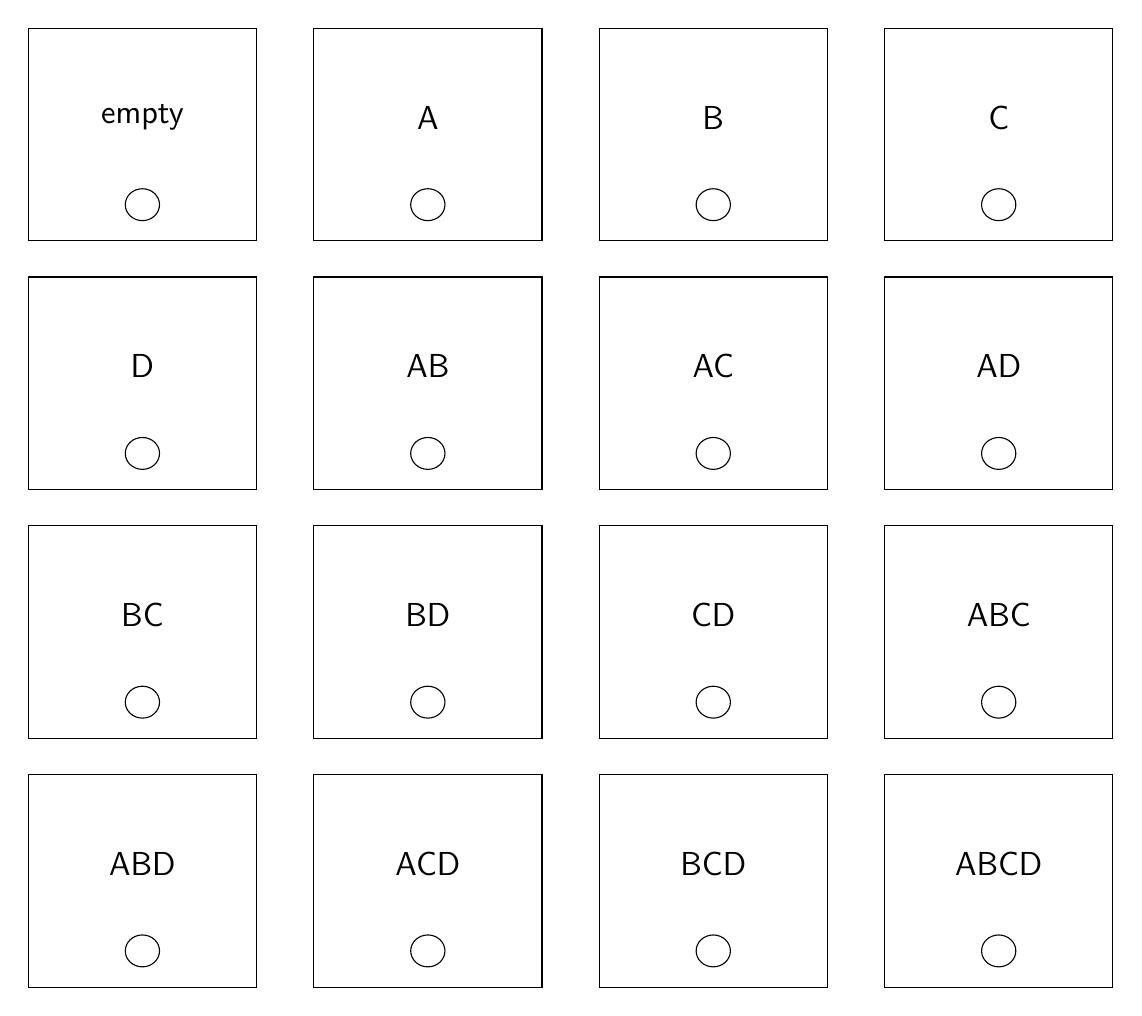
\begin{tikzpicture}[x=29mm,y=27mm]
\foreach \card [count=\i from 0] in {empty,A,B,C,D,AB,AC,AD,BC,BD,CD,ABC,ABD,ACD,BCD,ABCD}{\pgfmathsetmacro{\x}{mod(\i,4)*1.25}\pgfmathsetmacro{\y}{-floor(\i/4)*1.17}\draw (\x,\y) rectangle +(1,1);\node[font=\large] at (\x+.5,\y+.58){\card};\draw (\x+.5,\y+.17) circle (.075);}\end{tikzpicture}}
\begin{document}
A card holds a set of symbols; order does not matter. Use one copy of each card. An empty card has no symbols.

\problem{1}{Use the three-symbol deck. Choose as many cards as you can so every two chosen cards share a symbol. The empty card is forbidden. Mark your collection.}
\begin{center}\deckthree\end{center}
\lines{2}
\vspace{18pt}
\problem{2}{Make a collection as large as in Problem 1, with no symbol that appears on every chosen card. Every two cards must still share a symbol. Find one, or explain why it is impossible.}
\begin{center}\deckthree\end{center}
\lines{3}
\newpage
\problem{3}{Use the four-symbol deck. Make the largest collection in which every two chosen cards share a symbol. The empty card is forbidden. Explain why no larger collection can work.}
\begin{center}\deckfour\end{center}
\vspace{12pt}\lines{5}
\newpage
A trigger makes any card containing all of its symbols work. A card works if it contains at least one whole trigger.

\begin{center}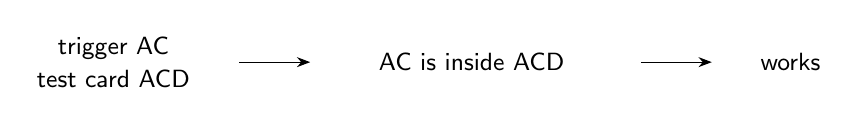
\begin{tikzpicture}[x=1cm,y=1cm]
\node[align=center] at (1.5,.5){\small trigger AC\\\small test card ACD};
\draw[-{Stealth}] (3.1,.5)--(4,.5);
\node[align=center] at (6.05,.5){\small AC is inside ACD};
\draw[-{Stealth}] (8.2,.5)--(9.1,.5);
\node at (10.1,.5){\small works};
\end{tikzpicture}\end{center}

\problem{4}{Use triggers AB and D. Mark every card that works. Then replace the triggers with A and BC, and mark the cards that work with the new triggers.}
\begin{center}\begin{minipage}[t]{.48\textwidth}\centering
\small AB and D\par
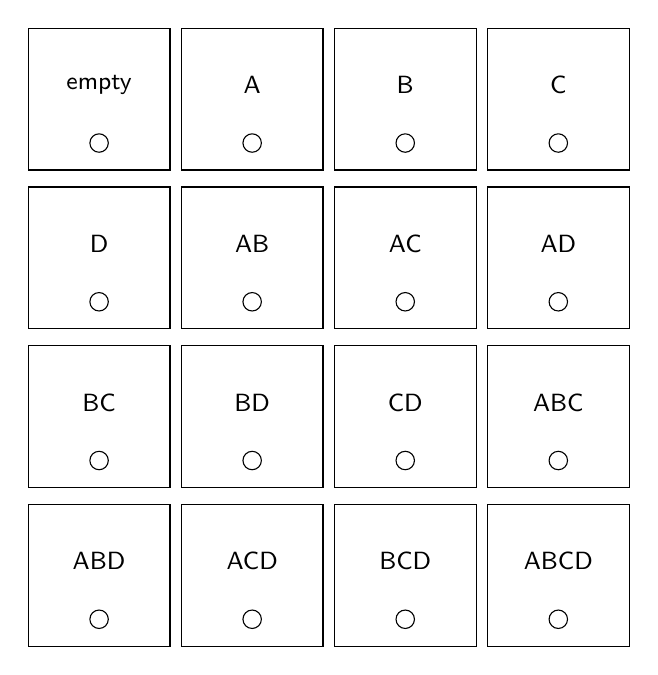
\begin{tikzpicture}[x=18mm,y=18mm]
\foreach \card [count=\i from 0] in {empty,A,B,C,D,AB,AC,AD,BC,BD,CD,ABC,ABD,ACD,BCD,ABCD}{\pgfmathsetmacro{\x}{mod(\i,4)*1.08}\pgfmathsetmacro{\y}{-floor(\i/4)*1.12}\draw (\x,\y) rectangle +(1,1);\node[font=\small] at (\x+.5,\y+.6){\card};\draw (\x+.5,\y+.19) circle (.065);}
\end{tikzpicture}\end{minipage}\hfill\begin{minipage}[t]{.48\textwidth}\centering
\small A and BC\par
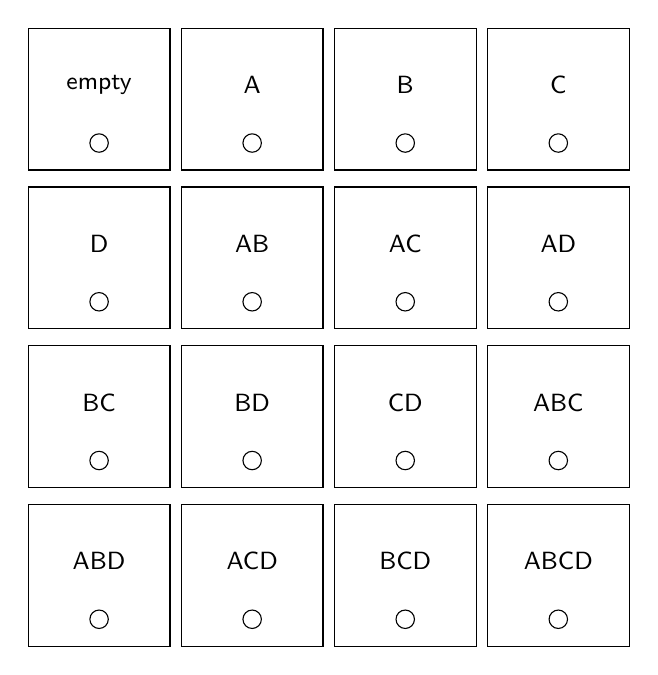
\begin{tikzpicture}[x=18mm,y=18mm]
\foreach \card [count=\i from 0] in {empty,A,B,C,D,AB,AC,AD,BC,BD,CD,ABC,ABD,ACD,BCD,ABCD}{\pgfmathsetmacro{\x}{mod(\i,4)*1.08}\pgfmathsetmacro{\y}{-floor(\i/4)*1.12}\draw (\x,\y) rectangle +(1,1);\node[font=\small] at (\x+.5,\y+.6){\card};\draw (\x+.5,\y+.19) circle (.065);}
\end{tikzpicture}\end{minipage}\end{center}

\problem{5}{These cards work: B, AB, BC, BD, ABC, ABD, BCD, ABCD, AC, ACD. Every other card fails. Find a set of triggers that gives exactly this rule, using as few triggers as possible.}
\lines{2}
\vspace{12pt}
\problem{6}{Invent a rule in which adding symbols to a working card never makes it fail. Mark the whole deck for your partner. Your partner must find every working card that stops working whenever any symbol is removed, and use those cards as triggers. Will those triggers always recreate the rule?}
\lines{2}
\newpage
\problem{7}{Use the three-symbol deck. Choose as many cards as you can without a nested triple: three different chosen cards with one inside the next inside the third. Nested pairs and the empty card are allowed. Explain why no larger collection can work.}
\begin{center}\deckthree\end{center}
\lines{2}
\newpage
\problem{8}{Use the four-symbol deck with the same rule: allow nested pairs and forbid nested triples. Make the largest collection you can, and find a way to show that no larger one works. The empty card may be chosen.}
\begin{center}\deckfour\end{center}
\lines{5}
\end{document}
